\documentclass[11pt,english]{article}
\usepackage{authblk}
\usepackage{graphicx}
\usepackage{xcolor}
\usepackage{amstext}
\usepackage{caption}
\usepackage{multibib}
\usepackage{etoolbox}
\usepackage{makeidx}
\usepackage{cancel}
\usepackage{tikz}
\usetikzlibrary{matrix,chains,arrows}
\include{epsf}
\usepackage{braket}
\usepackage{amsmath,amssymb,epsfig}
\usepackage{amscd}
\usepackage{mathrsfs}
\usepackage{dsfont}
\usepackage{array,boldline,makecell,booktabs}
%\usepackage[svgnames,table]{xcolor}
\usepackage{amsfonts}
\usepackage{authblk} 
%\usepackage{sectsty}
\usepackage{mathtools}
\usepackage{amsthm}
\usepackage[applemac]{inputenc}
\usepackage[english]{babel}
\usepackage{enumitem} 
\usepackage[]{latexsym}
\usepackage{caption}
\usepackage[CJKbookmarks, pdftex, bookmarksnumbered, bookmarksopen, colorlinks, citecolor=blue, linkcolor=blue]{hyperref}


%%%%%%%%%%%%%%%%%%%%%%%%%%%%%%%%%%%%%%

\definecolor{crimson}{rgb}{0.7, 0.08, 0.24}
\definecolor{blu}{rgb}{0.0, 0.18, 0.65} 



%%%%%%%%%%%%%%%%%%%%%%%%%%%%%%%%%%%%%%%%%%%%%

\renewcommand{\theequation}{\thesection.\arabic{equation}}
\newcommand{\be}{\begin{equation}}
\newcommand*{\email}[1]{\footnote{\texttt{#1}}}
\newcommand{\ex}{\text{ex}}
\newcommand{\red}{\text{red}}
\newcommand{\ee}{\end{equation}}
\newcommand{\bes}{\begin{eqnarray}}
\newcommand{\ees}{\end{eqnarray}}
\def\bean{\begin{eqnarray*}}
	\def\eean{\end{eqnarray*}}
\def\nn{\nonumber}
\newcommand{\dd}{\mathrm{d}}
\newcommand{\gi}{\mathfrak{g}}
\newcommand{\rig}{\rightarrow}
\newcommand{\Rl}{\mathbb{R}^3_\lambda}
\newcommand{\Rt}{\mathbb{R}^4_\theta}
\newcommand{\R}{\mathbb{R}}
\newcommand{\C}{\mathbb{C}}
\newcommand{\N}{\mathbb{N}}
%\renewcommand{\thefootnote}{\fnsymbol{footnote}}
\newcommand{\eqn}[1]{(\ref{#1})}
\newcommand{\p}{\partial}
\newcommand{\Tr}[1]{\:{\rm Tr}\,#1}
\newcommand{\add}[1]{\textcolor{blue}{}}

%\newcommand{\dd}{{\mathrm d}}
\def\baselinestretch{1.1}
\textheight 23cm \textwidth 17cm
\parskip 1ex
\oddsidemargin -5pt \evensidemargin 0pt \topmargin -50pt \jot = .5ex
\parskip 1ex

\renewenvironment{thebibliography}[1]
{\section*{References}\frenchspacing\small
	\begin{list}{[\arabic{enumi}]}
		{\usecounter{enumi}\parsep=2pt\topsep 0pt
			\settowidth{\labelwidth}{[#1]}
			\leftmargin=\labelwidth\advance\leftmargin\labelsep
			\rightmargin=0pt\itemsep=1pt\sloppy}}{\end{list}}

\numberwithin{equation}{section}
%\stepcounter{equation}

\captionsetup{tableposition=top,figureposition=bottom,font=footnotesize}

\input xy
\xyoption{all}


%%%%%%%%%%%%%%%%%%%%%%%%%%%%%%%%%%%%%%%%%%%%%%%%%%%




\begin{document}
	\title{TBD}
\author{TBD}  

\affil{ Institute for Theoretical Physics, University of Regensburg, 93040 Regensburg, Germany.}

\date{\today}

\maketitle

\begin{abstract}
	
\end{abstract}

\newpage


\section{Introduction}
It is widely believed that BFSS model \cite{Banks1997} has phase transitions \cite{Hanada2019}, \cite{Aharony2004}, and up to now it has been concluded that for the bosonic model, $D=9$ and $D=26$ spacetime dimensions the order of phase transition is one \cite{Bergner2019}. The model under consideration is a bosonic analogue  of the BFSS which has been extended to $d=D-1$ spatial dimensions and has a simple (Euclidean) action
\be 
S = \frac{N}{2\lambda}\int_0^\beta dt\ {\rm Tr}\left\{(D_t X_i)^2 -\frac{1}{2}[X_i,X_j]^2 \right\},~~i,j=1,\cdots,d
\ee 
It is an one dimensional model, which can be understood as a $d$ dimensional reduction of pure Yang-Mills theory living on $D$ spacetime dimensions. The covariant derivative acts as $D_tX_i=\p_tX_i-i[A_t,X_i]$ with $A_t$ being the gauge field.  The variables of the action are the matrices $X_i$ which enjoy a global $SO(d)$ symmetry that rotates them and in addition there is a $U(N)$ gauge symmetry associated with $A_t$.  The center symmetry is $U(1)$ under which the Polyakov loop is invariant. The latter is defined as  
\be 
\mathcal{P}:=\frac{1}{N}\Tr e^{i\int_0^\beta dt A_t},
\ee 
and is considered to be an order parameter that is associated with this center symmetry. If we denote as $\theta$ the eigenvalues of the Polyakov loop, then it is invariant under $\mathcal{P}\to e^{i\theta}\mathcal{P}$.  When this symmetry is broken (or restored), signals a phase transition and the main goal of this paper is to find the order of this transition for $D>36$. 

For $d=9$ we recover the bosonic BFSS and along the lines of gauge/gravity duality and for large $N$, there is a remarkable correspondence of this one dimensional model with a string theory living in 10 or 26 spacetime dimensions. The relevant string theory is IIA, which contains even number of $Dp$-branes.  This surprising duality relies on the fact that the degrees of freedom the matrix model are organised into $N\times N$ matrices which we called above $X_i$. The entries of the matrices have an intuitive interpretation that can be described as follows. The variables $X_i$ are hermitian and transform in the adjoint representation of the $U(N)$, where the latter being the gauge group of the action. Diagonal elements of $X_i$ are related with positions of $D0$-branes\footnote{That is because an open string starting and ending on a local D0-brane forms effectively a closed string that begins and ends at the same point in spacetime. In addition this effective closed string which is generated interacts with gravitation (closed string) modes. } in the gravity dual terminology and non-diagonal elements indicate interactions between the $D0$-branes.  Then the large $N$ limit corresponds to large matrices $X_i$, and the degrees of freedom contained in the entries of $X_i$ are of order $N^2$. The rest of the type IIA string theory ($D2$-and $NS5$-brane) can be reconstructed only from $D0$-branes with suitable polarizations and T-dualities \cite{Sen1998}.  


\textcolor{red}{**cite somewhere \cite{Gregory93}**}

In this paper, we wish to extend the results of  \cite{Bergner2019} to more than $D>26$ spacetime dimensions. Our ambition is to compare with the three-loop result obtained in  \cite{Morita2020} which predicts that higher order phase transitions should be happening after $D>36$. Of course it is understood that in these scenarios we are abandoning any connection with string theories and our only guidance is the matrix model and no known gravity duals whatsoever. The only statement we can make is that this particular model will be a $D-1$ dimensional reduction of a $D$ dimensional Yang-Mills theory because the latter can be written consistently in arbitrary spacetime dimensions.


\noindent 
There has been an analytic large $N$ prediction for critical temperatures in arbitrary dimensions in powers of $1/d$, with $d=D-1$ \cite{Mandal2010}. The results seem to propose that the critical temperature depends on the spatial dimensions as follows
\be \label{larged}
T_c=\frac{d^{1/3}}{\log d}\left[1+\frac{1}{d}\left(\frac{203}{160}-\frac{\sqrt{5}}{3}\right)\right]^{-1},
\ee  
and therefore we can determine the transition temperature for every $d$ as in table \ref{Tcrit}. 
	\begin{table}
		\centering
 \begin{tabular}{c|c|c}	
 	& d=40 &d=50\\
 \hline
 	$T_c$&0.915124&0.931965
\end{tabular}
	\caption{Critical temperature predicted from \eqref{larged}.}  
	 \label{Tcrit}
\end{table}

To determine the order of the transition we have to take $N$ to be sufficiently large because at this case the tunnelling between $\langle\mathcal{P}\rangle=0$ and  $\langle\mathcal{P}\rangle=\frac{1}{2}$ is exponentially suppressed by $e^{-\frac{N^2}{\lambda}}$. We expect that the Polyakov loop has a two peak signal in a scenario with first order transition, because the latter is characterized by a phase where $\langle\mathcal{P}\rangle=0$ , an intermediate unstable phase and a final phase where $\langle\mathcal{P}\rangle=\frac{1}{2}$. We see this in figure \ref{phaseorder}, where the corresponding phases are denoted with red, orange and blue lines. In a first order case, the unstable phase is also accompanied with negative specific heat. In the BFSS model, this unstable phase is connected to Schwarzschild black hole, but in our case there is no bulk dual interpretation available. On the contrary, a higher order phase has an intermediate stable phase between $\langle\mathcal{P}\rangle=0$ and $\langle\mathcal{P}\rangle=\frac{1}{2}$, denoted by a solid line. Therefore, in the simulations we expect to see an intermediate peak of the Polyakov loop, with the interpretation that the theory  stabilizes in this intermediate phase.   

\begin{figure}[h!]
	\centering 
	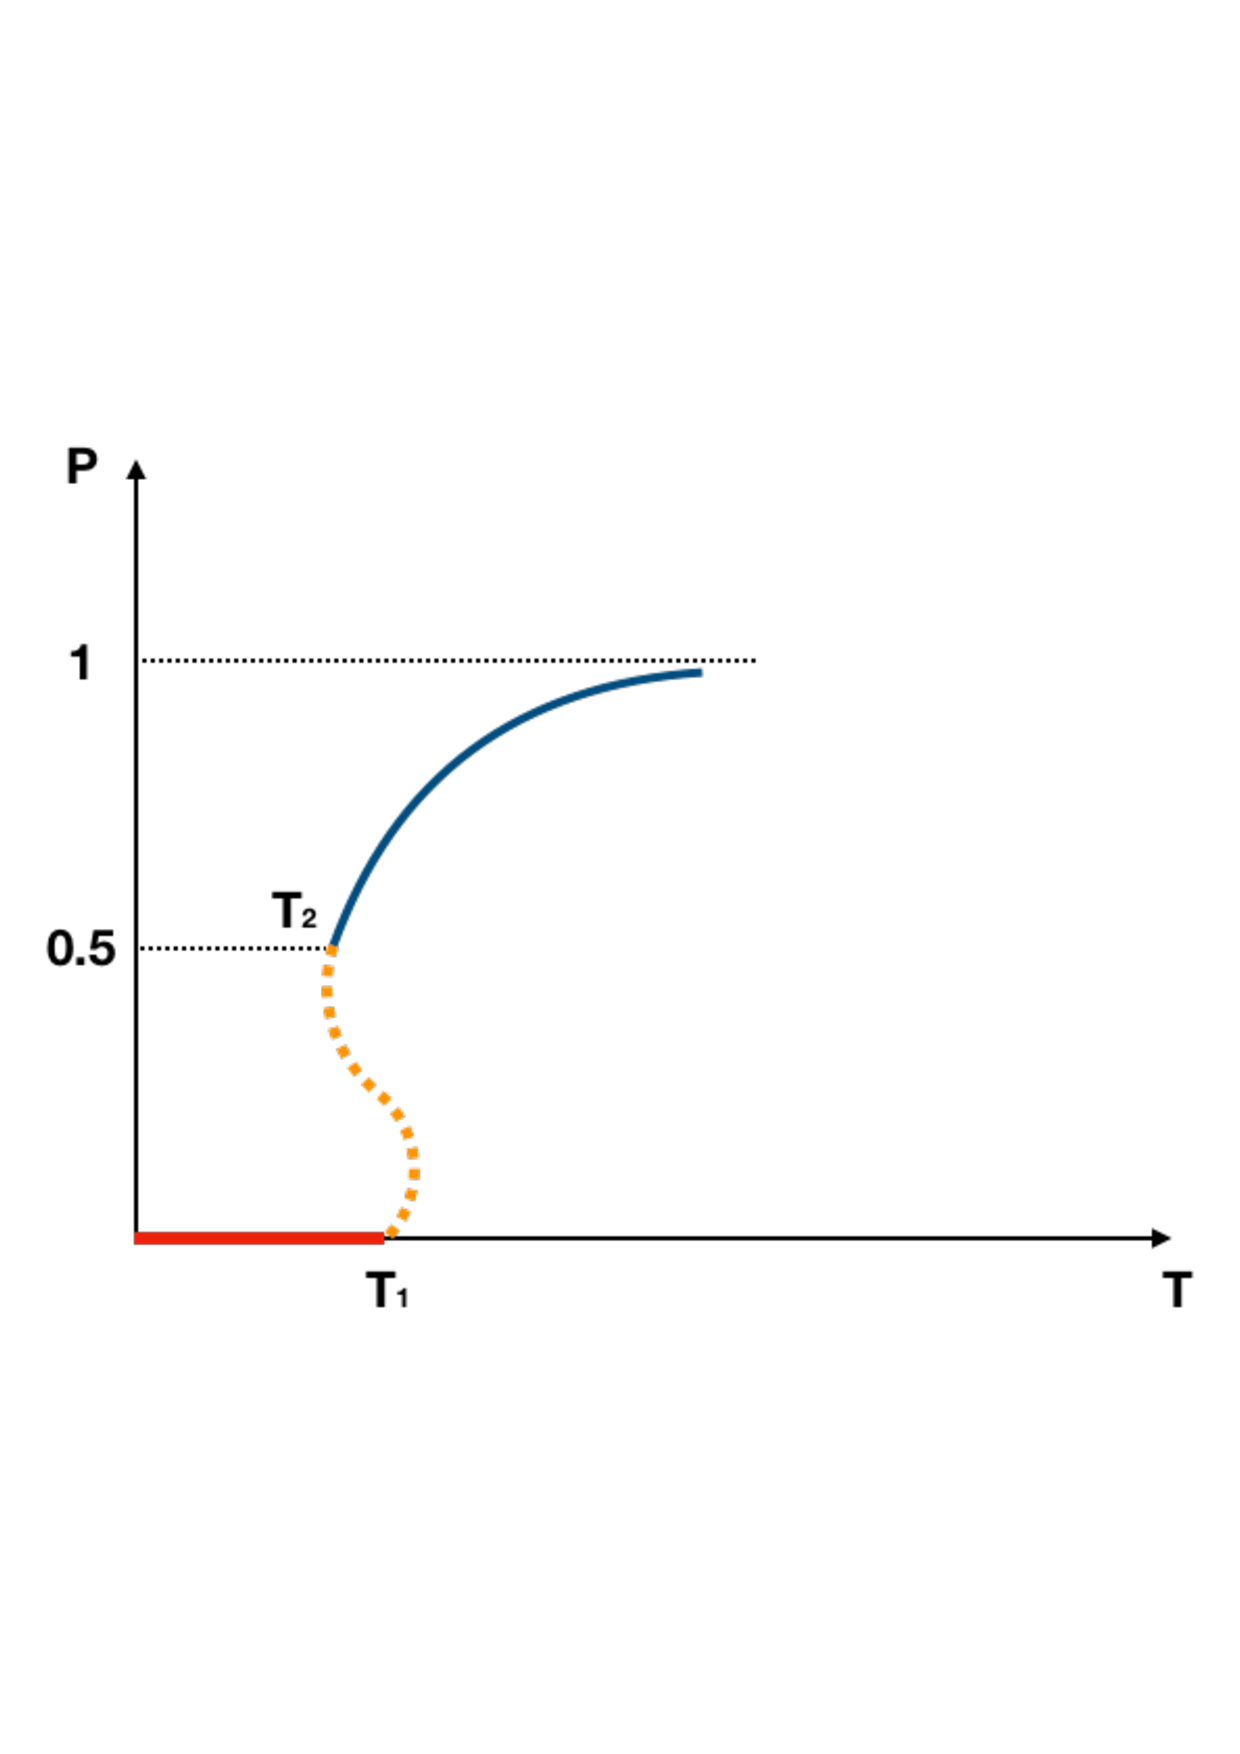
\includegraphics[scale=0.35]{first_order.pdf}
	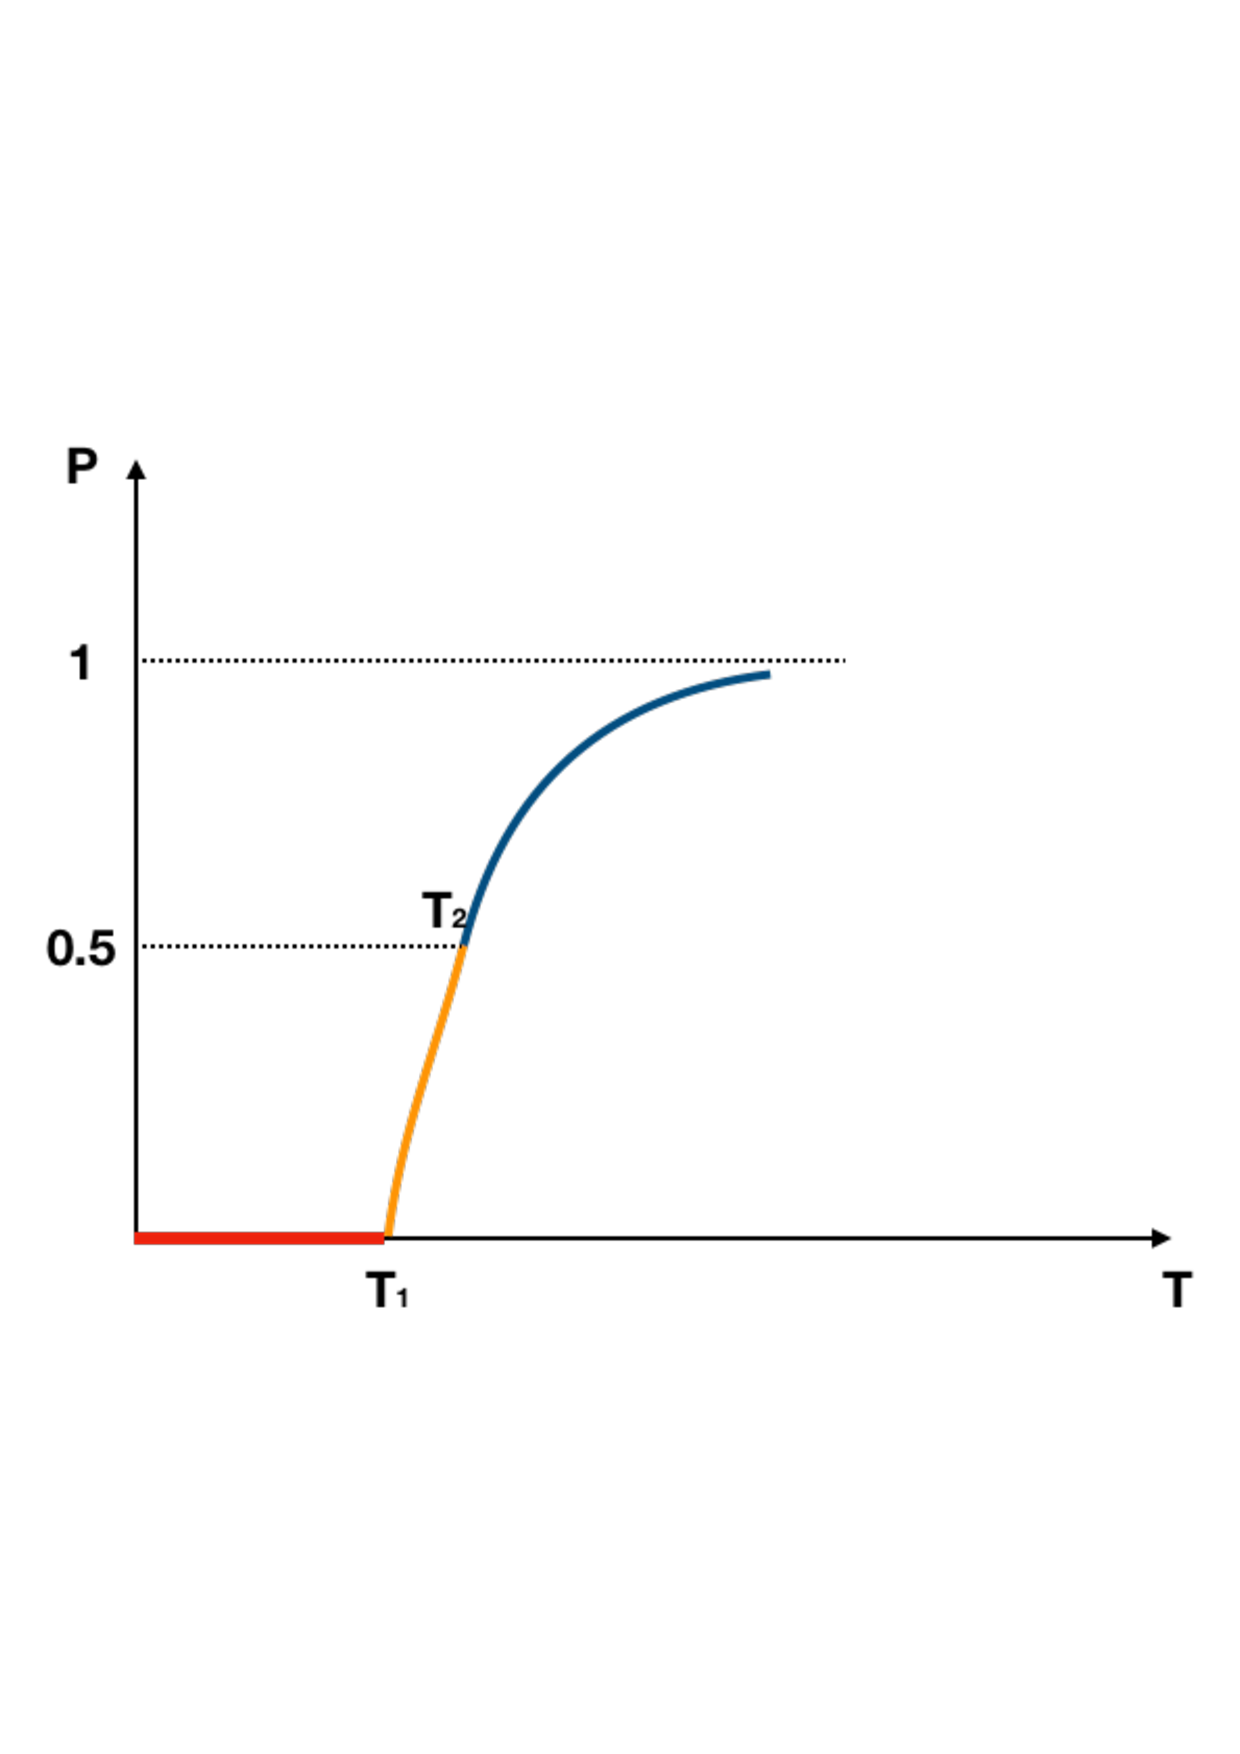
\includegraphics[scale=0.35]{second_order.pdf}
	\caption{Left: the first order transition with $T_2<T_1$ and the intermediate unstable phase denoted with dotted line. Right: higher order transition with a stable intermediate phase denoted with a solid line and $T_2>T_1$. }
		\label{phaseorder}
\end{figure}

 \section{Numerical results}
 We have performed a broad scan of temperatures for $D=40$ and $D=50$ starting from $T=0.1$ and up to $T=1.5$ with $N=32$ and $S=24$. Having located approximately the transition to be happening around $T_c$ we switched to $N=64,S=24$ and perform high statistics to see any possible signal structure of the Polyakov loop.
 
 \noindent 
 \textcolor{red}{Write the main result here!}
\subsection{d=40}


\begin{figure}[h!]
	\centering 
	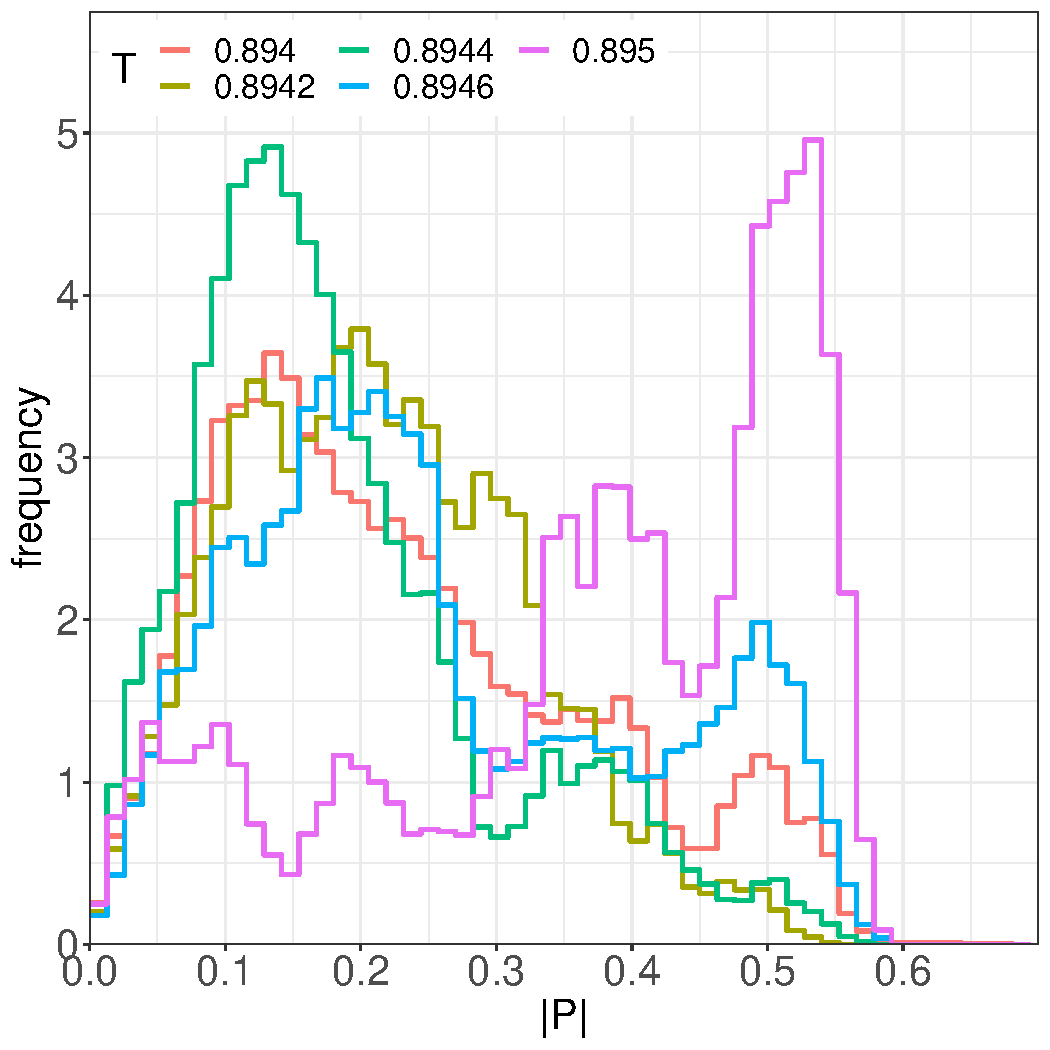
\includegraphics[scale=0.35]{Polyakov.pdf}
	\caption{The Polyakov loop around the transition temperature $T_c=0.8946$ for $N=64,S=24$.}
\end{figure}

\begin{figure}[h!]
	\centering 
	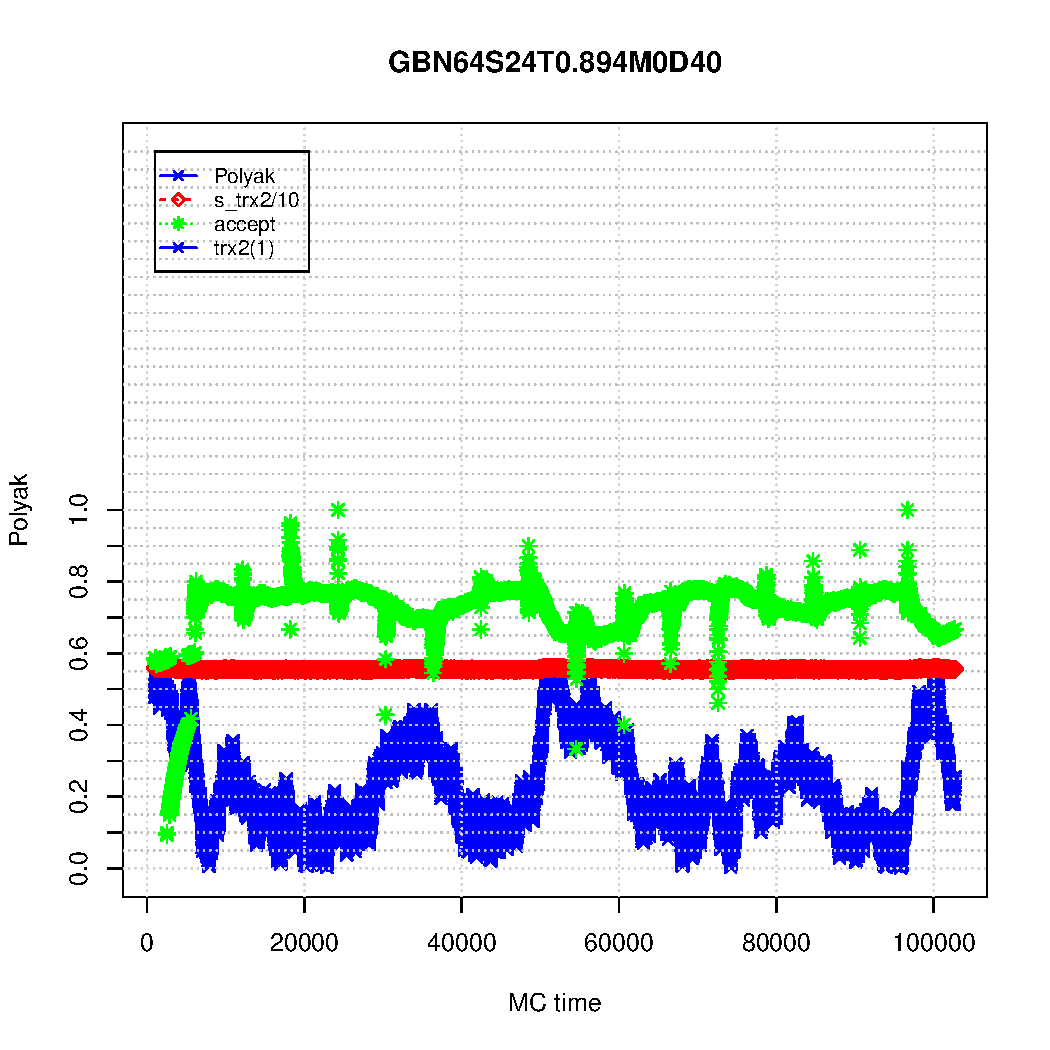
\includegraphics[scale=0.35]{pol_strx20894.pdf}
	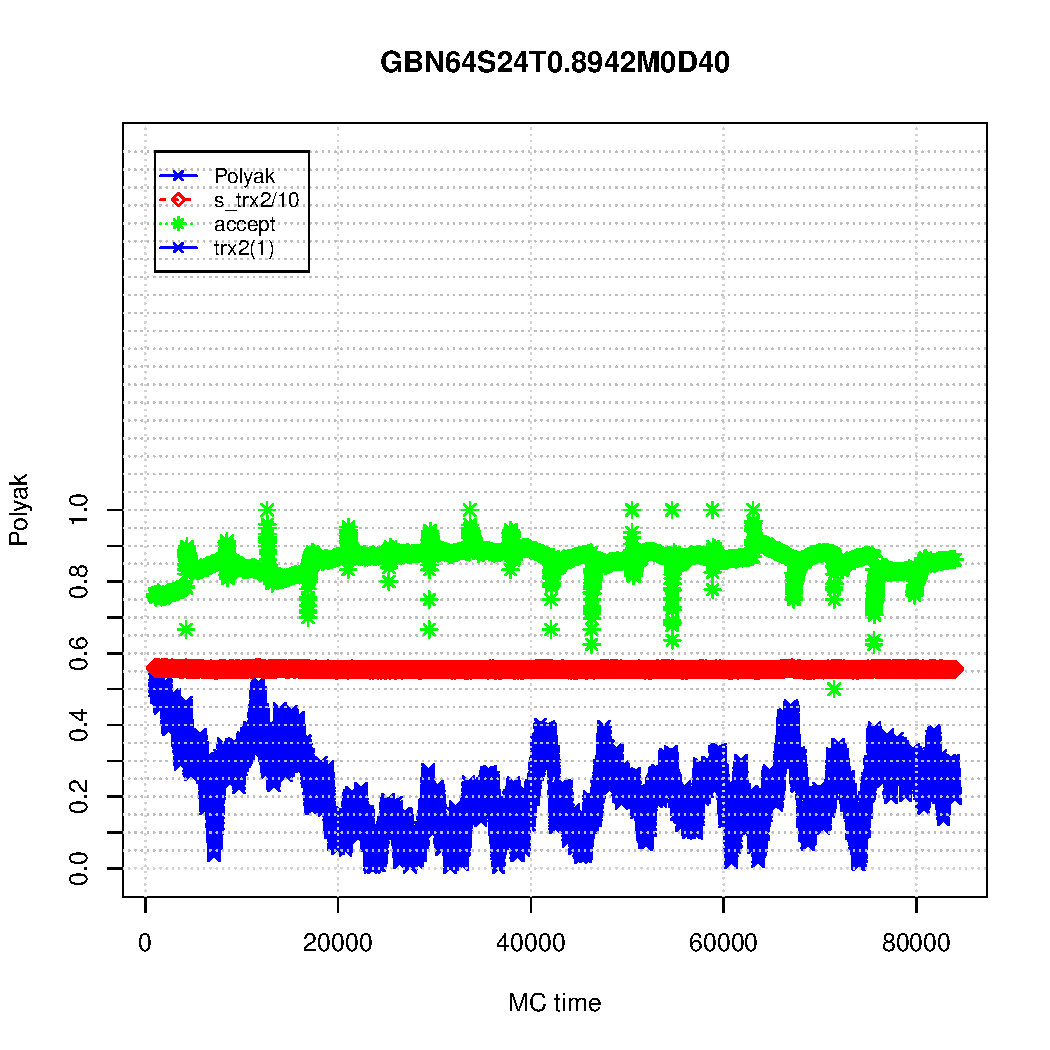
\includegraphics[scale=0.35]{pol_strx208942.pdf}
	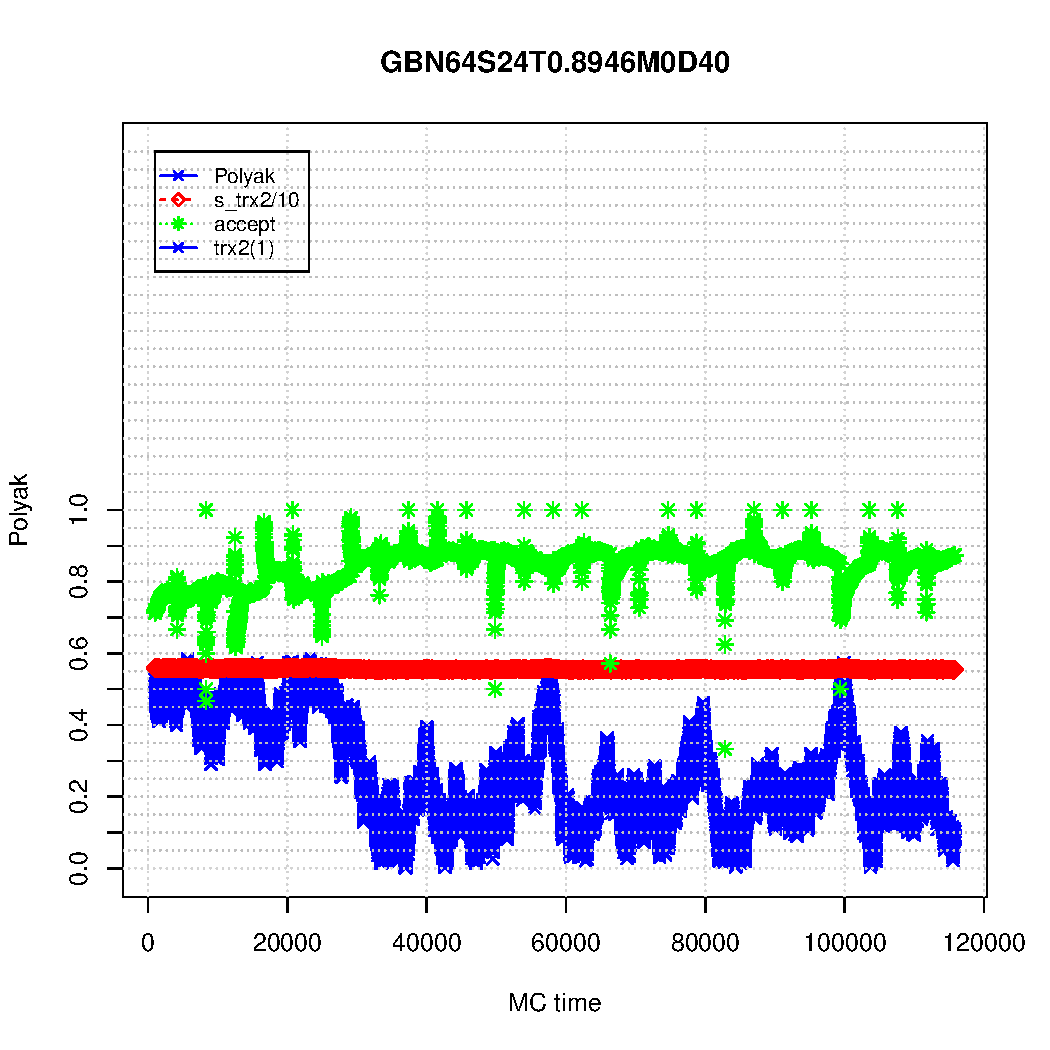
\includegraphics[scale=0.35]{pol_strx208946.pdf}
	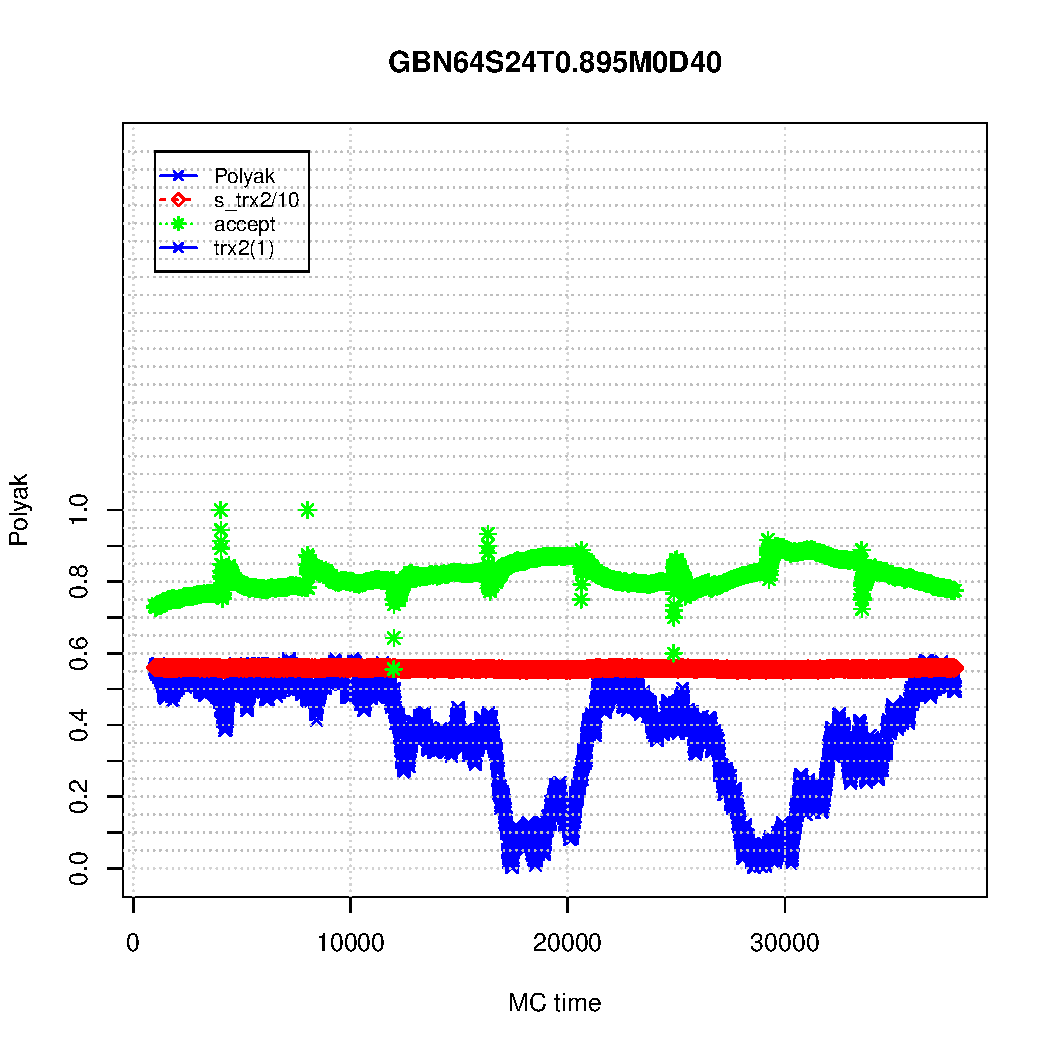
\includegraphics[scale=0.35]{pol_strx20895.pdf}
	\caption{Monte Carlo histories for different temperatures at $N=64, S=24$ configurations.}
\end{figure}
	
	%\nocite{}
	\bibliography{Matrix-related, D0-BMN}
	\bibliographystyle{utphysmendeley}
\end{document}
